\documentclass[]{final_report}
\usepackage{graphicx}
\usepackage{float}
\usepackage{hyperref}
\usepackage[backend=biber, style=numeric]{biblatex}
\usepackage{url}
%%%%%%%%%%%%%%%%%%%%%%
%%% Input project details
\def\studentname{Henry Frodsham}
\def\reportyear{2025}
\def\projecttitle{A Concurrency Based Game Environment}
\def\supervisorname{Felix Bradley}
\def\degree{BSc (Hons) in Computer Science}
\def\fullOrHalfUnit{Full Unit} % indicate if you are doing the project as a Full Unit or Half Unit
\def\finalOrInterim{Interim Report} % indicate if this document is your Final Report or Interim Report

\begin{document}

\maketitle

%%%%%%%%%%%%%%%%%%%%%%
%%% Declaration

\chapter*{Declaration}

This report has been prepared on the basis of my own work. Where other published and unpublished source materials have been used, these have been acknowledged.

\vskip3em

Word Count: 6577

\vskip3em

Student Name:  Henry Frodsham

\vskip3em

Date of Submission: 18/12/25

\vskip3em

Signature: Henry.f

\newpage
\tableofcontents
\newpage
\chapter{Abstract}

This project is a Real Time Strategy (RTS) Game that focuses on using concurrency to provide a Local Multiplayer (LCM) experience through split screen. This project's primary aim is to provide steady performance regardless of the game state or number of players. a Secondary goal of this project is to provide an unlimited progression system for players such that players can progress through the game regardless of how long they have been playing. \newline

Users of this project will be able to play with 1-5 people on the same device and display, with 1 player on a keyboard and mouse and up to 4 on different controllers. This project assigns regions of the display to each player and automatically adjusts the aspect ratio and size of pre-existing regions when a player connects or disconnects. \newline

The primary motivation for this project Is the poor performance of pre-existing RTS games, even those that focus solely on a single player experience. Other RTS games experience input delay and stuttering issues as the game progresses due to high unit counts and complex interactions between units; for example, Stellaris by Paradox Interactive is well known by the RTS community to slow down significantly in the late game, to the point that the game cannot be played. \newline

Another Motivation for this project is the lack of split screen multiplayer in the RTS genre. split screen is often exclusively implemented in First Person Shooter (FPS) and racing Games although even those genres have seen a decline in split screen as of recently [2]. This project aims not only to revive the once believed feature of Split Screen but also to introduce it to the RTS genre, RTS is by nature a game with complex interactions between players and the addition of face-to-face communication could overall benefit the experience. \newline

By combining the technical innovations of modern game development with older styles of gameplay featuring more face to face interaction, this project demonstrates that performant, social RTS gaming is both viable and practical.


\subsection{ Aims and Objectives of the project}

 \textbf{Primary Objectives} \newline

\textbf{ Performance Optimization} \newline

 - achieve and maintain a consistent frame rate that initially matches that of the end users maximum refresh rate, and doesn't drop below the minimum video frame rate of 23FPS for any given scenario 

 - maintain low input latency that doesn’t spike above 50ms in any given scenario but should match that of the end users minimum input latency initially

 - produce no additional input delay or lag spikes regardless of the number of split screen instances running

 \textbf{local multiplayer functionality} \newline

 - implement a split screen local multiplayer system that allows for 1-5 players to play the game simultaneously

 - develop a robust input handling system that provides consistent input delay across all game instances

 \textbf{long term stability} \newline

 - optimize storage and management of in game units to minimize the performance degradation for a large numbers of units

 - prevent memory leaks to ensure the games memory usage doesn’t increase after extended play time, ultimately resulting in a program crash

 \textbf{user experience} \newline

 - design a clean UI that is free of clutter and provides a consistent experience across different input devices

 - implement a sensible text size and UI scaling to ensure visibility regardless of how small a given split screen instance is 

\textbf{Secondary Objectives} \newline

\textbf{Comprehensive real time strategy game}\newline

 - survey and respond to real time strategy players preferences
 
 - implement a progression system that allows players to continuously progress regardless of game stage
 
 \textbf{Comprehensive player interaction} \newline
 
 - allow players to form beneficial agreements 
 
 - implement an enmity system that expands on rivalries between players
 
 - allow transfers of resources between players
 

\subsection{Technology choices}

\textbf{Programming language: } C++ 20 \newline
\textbf{Chosen Compiler: } MSVC (with Visual Studio 2022) \newline
\textbf{Rendering Engine:} Ogre3D 1.14.2 (not to be confused with Ogre3D-next) \newline
\textbf{Input Handling Library:} SDL2 \newline
\textbf{UI and Overlay Library: } Ogre Overlay Component \newline
\textbf{Concurrency Library: } <Threading> library in C++ included in std libraries \newline
\textbf{Dependency installation and linking: } vcpkg library integrated with Visual Studio 2022 \newline

\chapter{Project Timeline}
\section{Term 1 Timeline}
\subsection{planned timeline}
\textbf{ Week 1:} write unit tests following TDD and setup build dependencies \newline
\textbf{Week 2:} research efficient ECS and event architecture \newline
\textbf{Week 3:} research input methods for controller and keyboard \newline
\textbf{Week 4:} code central event bus and ECS registry class \newline
\textbf{Week 5:} code input listeners + initial world and instance class \newline
\textbf{Week 6:} code initial split screen functionality and implement event queue \newline
\textbf{Weeks 7:} code entity factories and create entity components for ECS \newline
\textbf{Week 8-9:} create initial game map with partial game functionality \newline
\textbf{Weeks 10-11:} prepare interim transcript and improve implementation for presentation \newline
\subsection{Development timeline}
Week 1:

Research efficient event architecture (moved up from planned Week 2)

Week 2:

Implement event bus and event queue architecture (significantly ahead of schedule - originally planned for Weeks 4 and 6)

Weeks 3-5:

Input handling system implementation (timing not explicitly stated, but completed successfully)

Achieved reconnection for controllers
Automatic device recognition and configuration

Weeks 5-7:
Overlay system implementation

Attempted Dear ImGui integration with Ogre3D
Encountered compatibility issues with ApplicationContextBase
Researched and implemented alternative overlay solution (Ogre Overlay)
Weeks 7-9:
config system implementation

universal config system for storing and reading JSON files with nlohmann JSON

Week 10:
refinements to implementation

thread safety update to event architecture
refined input system with more debug information available

Week 11:

Create ECS registry class with demo implementation (delayed from planned Week 4)
Create ECS components with ECS factory (delayed from planned Week 7)

Week 12:

Initial split screen functionality implemented (delayed from planned Week 6)

Automatic viewport creation on device connection
Dynamic viewport resizing
Consistent aspect ratio maintenance



Not Completed in Term 1:

Partial game functionality (originally planned for Weeks 8-9)
Deferred to Term 2 to allow for REA pattern integration
 
\section{Term 2 Timeline}
\textbf{Week 1: revisit term 1 implementation, refactor threading model and class communication} \newline
\textbf{Weeks 1-2: Research REA implementations, implement a basic scenario with multiple entities that can perform basic actions. } \newline
\textbf{Weeks 3-4: create a game world and a basic test scenario where each player is given starting units and starting territory} \newline
\textbf{Weeks 4-5: model and create simple REA actions for taking territory, attacking units, placing units.} \newline
\textbf{Weeks 6-7: create an undecorated UI, including context menus for actions that change depending on where the cursor is. settings and main menu screen} \newline
\textbf{Weeks 7-8: perform market analysis on experienced real time strategy players and implement suggestions as prototypes} \newline
\textbf{Weeks 8-9: perform user testing with prototypes to produce an unrefined game as the basis for the finished project} \newline
\textbf{Weeks 9-12: produce a shader complimenting a simplistic art style, implement a refined UI} \newline
\section{Retrospective}
Over the development period in Term 1 there where some major differences between the planned timeline and actual development timeline. specifically, \newline
	- earlier development of event architecture fundamentals \newline
	- 2 week delay to implementing an overlay system \newline
	- delay to split screen functionality \newline
	- absence of partial game functionality \newline

Term 1's development has brought to my attention that more careful analysis of planned technologies is required. Specifically, investigating implementations in other projects using similar technologies to me and which prerequisites are required or which existing technology could conflict. Another lesson learned from term 1's development is that more consistent contribution to reports and documentation is required in term 2's development, this way the CFD can easily be used to identify potential race conditions or design flaws.

Despite these delays to the projects timeline, This project has reached a satisfactory end result for term 1. Large architectural groundwork has been completed, making way for development in term 2 along with recognizing REA as a new proven beneficial technology.


\newpage
\chapter{Technical Literature Survey}
\section{Core Real time Strategy Game Architecture}
\subsection{Entity Classification and Entity Interactions}
RTS games are heavily focused on “units” such as friendly soldiers or a farm that produces the player food every x amount of time. Each “unit” within an RTS game is highly varied in their behaviour but may have shared or common behavior between each other such as a position on the screen and a 3D model. \newline

A major challenge faced during the development of RTS games is storing and handling entities differently according to their behaviour, without an efficient method to store and compute the behaviour of large numbers of entities it causes major performance concerns as the number of entities increases. Despite there being pre-existing methods to tackle this problem it’s still common to see an “end year” or a “victory year” implemented within RTS games to prevent the number of units growing too large. The primary reason for RTS Games still implementing a limit to game time is the inclusion of highly detailed 3D meshes where unnecessary. \newline

One popular choice used for entity storage in the development of RTS games is ECS (entity component system) since it not only provides efficient storage but provides the perfect solution to classify modular entity behaviour through its component system. ECS's component system allows developers to modularize entities into specific behaviours that can easily be reused or removed from that entity to modify its behaviour. \newline 

ECS is a powerful choice for Real time strategy games due to entity and component access being constant O(1) time, this means that the time complexity of managing entities doesn't increase with more added entities. the reason for ECS being O(1) time is due to its employment of sparse set, a data structure consisting of two arrays with one sparsely filled with indexes and another containing densely packed arrays. the indexes in the first array of indexes point to a densely packed list in the second array, Here's a visual representation of sparse sets operation. \newline

\begin{figure}[H]
	\centering
	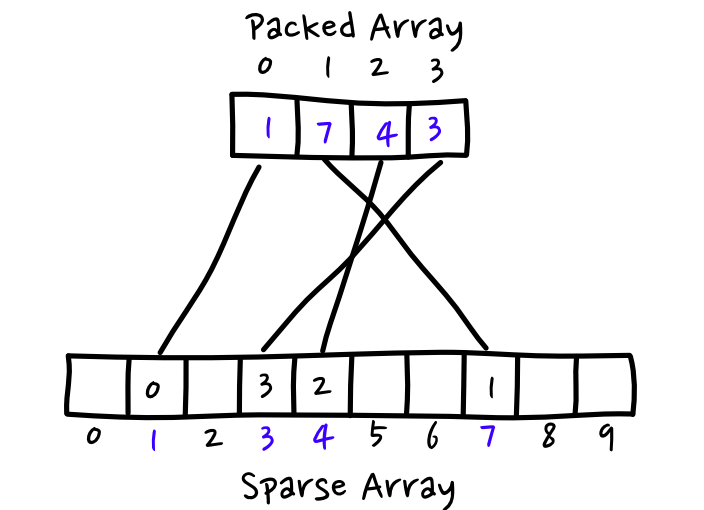
\includegraphics[width=0.7\linewidth]{screenshot001}
	\caption{sourced from Reference [1]}
	\label{fig:screenshot001}
\end{figure}
Its important to note that that elements in the sparse array contain indexes pointing back to the dense array, this is used in ECS to achieve O(1) time complexity for both retrieving the entity from a given component and for retrieving a component from a given entity.
This diagram however does not properly illustrate how ECS implements sparse sets in its component system, Here's a diagram showing how sparse set in a practical implementation of ECS would actually look like. \newline
\begin{figure}[H]
	\centering
	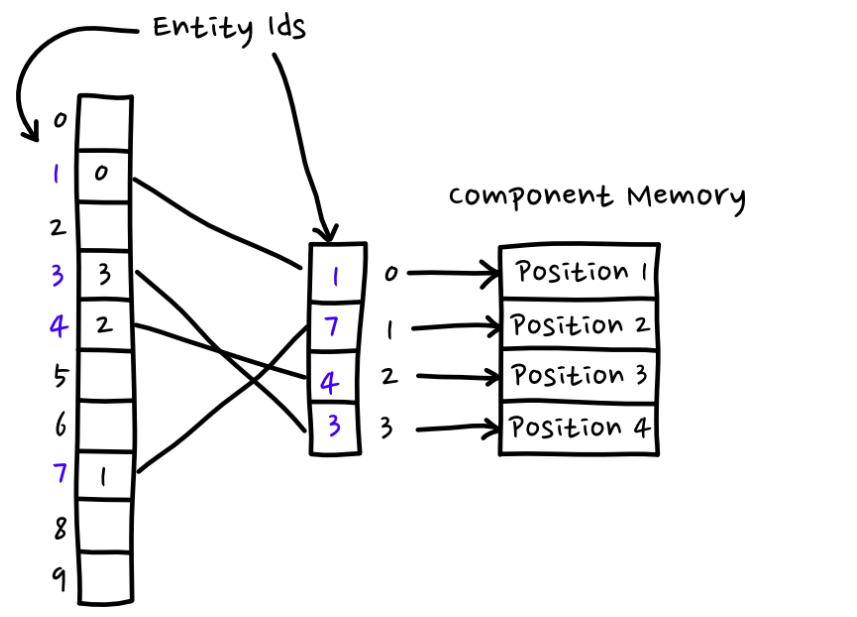
\includegraphics[width=0.7\linewidth]{screenshot002}
	\caption{sourced from Reference [1]}
	\label{fig:screenshot002}
\end{figure}
This diagram shows the relationship between the sparse set and a specific component and proves O(1) lookup time. its easy to assume that having 2 components would mean iterating over 2 different components however this isn't actually the case and instead a new sparse set is made for each component. \newline



However, evaluating actions between entities is still a major issue faced by RTS strategy games. when the number of units increases it also increases the amount of units implicated by a specific action thus exponentially increasing the processing time required.  \newline

 REA (Resource entity action) addresses this issue by modelling entity actions as resource exchanges that use Transformation matrices to evaluate the resulting resources that affected entities have after a given action. One example of a situation that REA is useful in is if two units in an RTS game attack each other then a Transformation matrix is used to calculate the resulting health of both entities. REA pattern has been proven to provide a performance edge over implementations without [2]. \newline
 
 as mentioned before, REA uses a matrix to evaluate actions as resource exchanges but this isnt always suitable for every entity interaction. REA is primarily used for menial calculations that are most commonly run and don't have complicated conditions or implications, for instance a RTS game might use REA to calculate how much money a factory unit should produce each second since the conditions for which are likely basic. \newline
 
 

\subsection{Split Screen Multiplayer Approaches }

LCM (Local cooperative multiplayer) involves having multiple players able to play on the same device, each player receives a portion of the screen that they can independently control with an input device. LCM is rare especially in the RTS (real time strategy) genre, LCM is most common in the FPS or racing genre although recently its seen a decline in those genres aswell. One reason for this decline is the relative difficulty compared to single player games, most game developers avoid LCM simply because its expensive and time consuming to implement. \newline
LCM provides significant technical difficulty when managing input devices between players since each device must be distinguishable and be able to be read at the same time. some LCM games combat this issue by simply not having multiple input devices and instead having players share a keyboard, although this approach is only applicable to simplistic games not requiring a cursor or camera control. \newline

LCM games that do use separate input devices typically do so using an input library that can distinguish between input devices, the most popular being the GameInput library for windows and xbox [4]. SDL is also a popular choice for cross platform compatibility since SDL2 handles platform specific code automatically without the need of platform specific Keymaps. \newline

There are differing approaches to how regions of the display are divided in LCM play, the standard approach is fixed size segments such as in the console editions of Minecraft although a unified view and distance based splitting also being approaches made by game developers. \newline


\subsection{How I chose my implementations of ECS}
ECS can be implemented via various libraries in C++, two notable ones are Flecs and Entt. Entt uses solely sparse set to store entities whereas Flecs can use either sparse set 

Flecs has an advantage over Entt in terms of ease of use due to its query engine, making multiple entity and component retrievals easier to manage. Flecs is also included in the std library in c++ meaning it has the added advantage of not adding extra dependencies to my project.

However the main criteria im concerned with is their efficiency and space overhead. below is a table showing the space and time complexities of both libraries.

\textbf{Time Complexity} \newline
\begin{table}[!h]
	\centering
	\begin{tabular}{|l|c|c|}
		\hline
		\textbf{Operation} & \textbf{EnTT (Sparse Set)} & \textbf{Flecs (Archetype)} \\
		\hline
		\multicolumn{3}{|c|}{\textit{Entity Operations}} \\
		\hline
		Create Entity & $O(1)$ amortized & $O(1)$ \\
		\hline
		Delete Entity & $O(1)$ amortized & $O(1)$ \\
		\hline
		\multicolumn{3}{|c|}{\textit{Component Operations}} \\
		\hline
		Add Component & $O(1)$ amortized & $O(n)$\footnote{$n$ = entities in source archetype} \\
		\hline
		Remove Component & $O(1)$ amortized & $O(n)$\footnote{$n$ = entities in source archetype} \\
		\hline
		Get Component & $O(1)$ & $O(1)$ \\
		\hline
		Has Component (Check) & $O(1)$ & $O(1)$ \\
		\hline
		\multicolumn{3}{|c|}{\textit{Query/Iteration Operations}} \\
		\hline
		Iterate All Entities & $O(n)$ & $O(n)$ \\
		\hline
		View/Query Iteration & $O(n)$ & $O(n)$\footnote{With cached query} \\
		\hline
		Uncached Query Iteration & N/A & $O(A)$\footnote{$A$ = number of matching archetypes} \\
		\hline
		Create Cached Query & N/A & $O(E \log E)$ or $O(E)$\footnote{$E$ = total entities} \\
		\hline
		Create Uncached Query & N/A & $O(1)$ \\
		\hline
		Lookup Entity by Name & $O(1)$ & $O(1)$ \\
		\hline
		Component Registration & $O(1)$ & $O(1)$ \\
		\hline
	\end{tabular}
	\caption{Time Complexity Comparison - EnTT vs Flecs sourced using [5] and [6]}
\end{table}

\textbf{Space Complexity} \newline
\begin{table}[!h]
	\centering
	\begin{tabular}{|l|c|c|}
		\hline
		\textbf{Data Structure} & \textbf{EnTT (Sparse Set)} & \textbf{Flecs (Archetype)} \\
		\hline
		Entity Storage & $O(E)$\footnote{$E$ = max entity ID} & $O(E)$\footnote{$E$ = number of entities} \\
		\hline
		Component Storage & $O(E \cdot C)$\footnote{Sparse per component} & $O(E)$ (dense per archetype) \\
		\hline
		Sparse Index & $O(E)$ per component & N/A (uses archetype structure) \\
		\hline
		Archetype Storage & N/A & $O(A \cdot C)$\footnote{$A$ = archetypes, $C$ = avg components} \\
		\hline
		Query Cache & N/A & $O(Q \cdot A)$\footnote{$Q$ = queries} \\
		\hline
		Total Memory (avg case) & $O(E + E \cdot C_{avg})$ & $O(E + A \cdot C_{avg})$ \\
		\hline
		Total Memory (worst case) & $O(E \cdot C_{max})$ & $O(E \cdot C_{max})$ \\
		\hline
	\end{tabular}
	\caption{Space Complexity Comparison - EnTT vs Flecs sourced using [5] and [6]}
\end{table}



as can be seen on the table, Entt has the clear advantage in terms of speed and component overhead. whilst Flecs would be significantly easier to use and manage, my final choice for this project was Entt due to the performance focus of this project and any performance edge gained for such a critical architectural feature of this project must take priority.
\subsection{my use of ECS in this project}
ECS entities within this project are created using a factory pattern, where entities being created are split into their individual components then added in serial to the ECS registry to form the complete entity. below is a control flow diagram showing this process for the example cube.

\begin{figure}[H]
	\centering
	\includegraphics[width=0.7\linewidth]{"../Cube creation example"}
	\caption{a CFD of the example cube creation process}
	\label{fig:cube-creation-example}
\end{figure}

the example cube is made up of 2 ECS components. an OgreComponent and a MeshComponent, the OgreComponent contains an ogre scenenode (a universal object for any ogre entity) and the MeshComponent contains the mesh file path.
\subsection{how i chose my approach to split screen}
My chosen approach to split screen in this project is fixed size screen regions. Whilst a unified view of the game world would have been an acceptable choice for this project i decided against it to prevent confusion with multiple user interfaces appearing simultaneously on the same camera, the lack of individual camera control was also a factor considered since users wouldn't be able to focus in on specific game events. fixed screen sizes however do mean that a large display size is required to comfortably play with 4 or more players, careful design will be required for future development of this project to maximise accessibility for smaller displays.

\section{Concurrency in game Development}
\subsection{threading models}
threading models in game architecture is a fundamental architectural decision when designing games, threading models dictate how processing load is spread across different threads and thus spread across cpu cores. since modern CPU's almost always contain more than 1 core with most having 4-8, it's critical that these cores are utilized effectively to improve performance in game design. Single core dependence is a common issue faced in the RTS genre where only one cpu core is utilized due to architectural limitations, one example of this is Stellaris by Paradox Interactive which is known for poor late game performance since only 1 core is processing large numbers of game units.

one common approach to threading in game architecture is thread pooling, thread pools split tasks over a finite number of worker threads through a shared worker queue. one issue with thread pooling however is that two threads may access the same game resource at the same time since two threads could take a task accessing the same data. thread pooling is an extremely common approach in game design as if implemented correctly can ensure consistent core utilization across each cpu core.

another approach to threading models in games is the actor-entity model where each game object (actors) maintains their own internal state and reacts to messages. this approach avoids race conditions entirely as each thread processes actors without direct memory sharing meaning two threads will never access the same memory location. this approach does however introduce latency and ordering challenges since messages may arrive late or out of order.

\subsection{race condition avoidance}
Race conditions occur when two different threads attempt to enter the critical region at the same time e.g two threads access a variable at the same time. Race conditions are problematic since one thread could potentially read the value in the critical region whilst the other thread writes to the variable, causing thread 1’s read value of the variable to be incorrect.
Race conditions can be avoided in multiple different ways, the most notable being mutex locks where once a thread accesses a critical region it will lock access for other threads until it has exited. However, this creates problems of its own since one thread will be stuck waiting to enter the critical region and will sit idle until the other thread exits.

Another popular way game developers avoid race conditions is through Event architecture. Event architecture is composed of two main parts, Event Bus's and Event Queues with Event Bus's notifying subscribing functions immediately after an event is published then Event Queue's queuing up events to be processed in serial after its dispatch method is called. Event queues avoid race conditions by processing critical region accessing tasks one after the other thus preventing two accesses at the same time. 

\subsection{My approach}
My chosen Thread model for this project is thread pooling, each game instance will be assigned a thread that are synced at the end of each frame then reused for the next frame. Due to the nature of Ogre3d only being safely accessible from one thread i have seperated task queues into a local queue and a global queue. the local queue runs thread safe events only accessing that game instances data then the global queue is used to process non thread safe events such as moving a viewport.

whilst it can be said that Ogre3d only being able to be accessed from a single thread is a limitation of my project its important to note that down to a fundamental level GPU's run tasks in serial so issuing rendering commands in a multithreaded environment provides no significant advantage.
\section{Graphics/Rendering Engines}
\subsection{Comparison of commonly used Engines}
Game engines are systems that abstract complex rendering from developers. There are a variety of commercial and open source game engines available, each providing differing levels of abstraction. some well known choices being unreal engine and unity which are both considered heavyweight game engines since they abstract processes such as entity storage and concurrency. Open source and lightweight game engines are also widely used, the most popular being GoDot which abstracts considerably less than heavyweight game engines.

Whilst heavyweight game engines are the standard for large game development companies, they do introduce significant overhead and performance implications. The most notable example of this is with Unreal Engines 5's Nanite system for high detail meshes [3], some games use this system unnecessarily introducing no real visual fidelity benefit but causing significant performance degradation. One recent example of this is Borderlands 4, which has been criticized for poor performance on even high end hardware.

Lighter weight game engines are the clear choice when it comes to games focusing on performance. lighter weight game engines run with less overhead and systems such as entity storage are added via stand-alone libraries, following the "pay for what you use" principle. most game developers however still opt for heavyweight game engines despite a lack of real need for them, usually due to ease and thus cost of development. 

\subsection{Overlay and GUI Libraries}
Overlay systems are Rendering libraries that render 2d text or shapes over a 3d game world. Overlay systems are used by developers to show debug information such as current input device states and are also used to create GUI's for use by an end user. 

One popular Overlay system used in Game development is Dear Imgui. Dear Imgui is widely used to create debug overlays since it abstracts creating text inputs or drop down menus from developers, 
allowing sophisticated debug overlays to be created easily and conveniently by developers. Dear imgui is however unsuitable for creating a modern GUI for end user's since it's appearance is designed strictly to create tools, in addition to this Dear Imgui redraws the entire ui every frame which is unnecessary for menu buttons that largely remain static.

below is a picture of Dear Imguis UI
\begin{figure}[H]
	\centering
	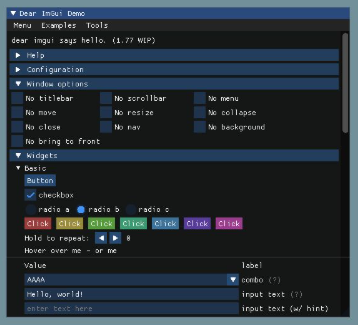
\includegraphics[width=0.7\linewidth]{screenshot003}
	\caption{}
	\label{fig:screenshot003}
\end{figure}

Another popular option is CEGUI, which is primarily used for GUI's.

\subsection{My Approach}
My chosen Overlay system is the Ogre Overlay library, which is natively included in Ogre3d. due to Ogre Overlay being part of Ogre3d's ecosystem it allows for convenient integration into this project, this has several benefits such as being able to create unique overlays for each viewport and inclusion within Ogre3d's rendering pipeline. Ogre Overlay is simplistic in terms of features such that Buttons and drop down menus must be created manually, although this means that a GUI library can be produced that is more specialised for this project's needs.

I had initially planned to use Dear Imgui to produce a debug overlay for this project, however due to unforeseen issues with integrating Dear Imgui with ogre i now use Ogre Overlay exclusively.
 
\chapter{implementation so far}
\section{concurrency}
This project has implemented Concurrent execution of each game instance, each game instance thread is managed using the thread pooling pattern. 

due to the current project state, each game instance thread is currently taking on a very small amount of processing responsibility. however, the system infrastructure required to distribute complex processing across game instance threads is implemented and once the project reaches a more complete state then the advantages of multi threading becomes more apparent.
\section{input handling}
This project has implemented Input handling using SDL2 with concurrent input translation happening for each game instance. both controller and keyboard+mouse input is read, both types of input device's activity is translated to a cursor position on the screen and a camera angle (changes based on relative movement).

Another implemented feature for input handling in this project is disconnect handling. if a controller is disconnected whilst the project is running then the controller is reconnected to the correct game instance once the device reconnects. 

however, the disconnect handling is not yet complete due to a limitation with SDL2 where generic controllers cant be distinguished on the basis of vendor and product id. the finalised disconnect handling will have a text prompt that prompts a user that has disconnected to press a button on their controller.
\section{ECS}
This project has implemented ECS for storage and classification of game objects. visible game objects such as the demonstration cube can easily be created through entity templates that construct ECS entities using a factory design pattern. the created ECS entities are automatically linked to ogre3d such that they are visible from a viewport.

the universal Entity components have been created storing pointers to Ogre objects to allow for easy modification of the stored entities.  

\section{Project CFD}
\chapter {deployment}
\section {deployment prerequisites}
 
\textbf{at a bare minimum you should possess:} \newline
- an x64 based cpu 
- an operating system compatible with OpenGL or DirectX
- at least one games controller to test the split screen functionality
- a modern dedicated GPU, preferably one with more than 4gb of video memory.
 
\textbf{additionally, before deploying this project please ensure you have installed and configured the following:} \newline
-  Visual studio Community edition 2022
-  the vcpkg component of visual studio 


details on how to install and configure the above can be found in the deployment video provided in the git repository.
\section{deployment instructions}

* open product.sln (if a retarget prompt appears then refer to deployment perquisites) \newline
* this project uses cpplint in pre build events, run "pip install cpplint" (important that this is done in the vs python command prompt and not a regular command prompt) \newline
* you'll be presented with 3 different projects in visual studio, "product" is a static lib and "tests" + "application" is an exe \newline
* before compiling, configure "multiple startup projects" and make sure that the static lib isn't run but the other 2 are \newline
* clean then rebuild all using visual studio, vcpkg will download and install dependencies (usually takes ~2-~3 hours) \newline
* please note that if the first run fails it means that vcpkg automatic linking failed. as a fallback, post build events will copy all required DLLs to the output dir meaning the second run wont fail. \newline
* if you get a fatal error (code 5000+) on runtime ("failed to link plugin OpenGL") and a subsequent ("failed to set DirectX as a fallback") then you must install either of them then restart. \newline
* *VERY IMPORTANT* if you are running my project from inside visual studio you must change the debugging directory (working directory in the debugging section) for each individual project (application, product, tests)  to \$(OutDir) (must be uniform between projects), prebuild events will copy the right ogre config to the outdir so please keep in mind if you decide to build my project to a different directory (outside of visual studio) then you need to recreate this behaviour.\newline



\chapter{Software engineering methodologies}
\section{testing environment}
This project uses the Doctest C++ library for unit testing with Cpplint to check for google c++ style compliance.To test for memory leaks and concurrent performance within my project im using the native visual studio debugger with Open Hardware Monitor to check core utilization.

This project is tested on 2 different computers

\textbf{Primary development computer } \newline
\textbf{Operating System:} Windows 11 Home edition \newline
\textbf{CPU:} Ryzen 9 9950X3D \newline
\textbf{GPU:} Nvidia RTX 5090 \newline
\textbf{RAM:} 64GB DDR4 \newline
disk running and storing project: Nvme SSD \newline

\textbf{secondary development computer} \newline
\textbf{Operating System:} Linux Mint with Wine installed \newline
\textbf{CPU:} Ryzen 7 3700x \newline
\textbf{GPU:} AMD Radeon 7700XT \newline
\textbf{RAM:} 16GB DDR4 \newline
disk running and storing project: standard sata SSD \newline

\textbf{both running at factory clock rates} \newline

\section{Use of TDD}
This project was developed using a structured and methodical approach to modern software engineering practices.using industry standard system design from both a Game development and a concurrency standpoint, My Deployment process is also streamlined for rapid deployment with unit testing done to ensure correctness. Unit tests are automatically run alongside this project when run inside visual studio meaning i can easily identify if a new feature has affected previous functionality, alongside this cpplint is run as a prebuild event to check for google c++ standard compliance.
\section{system architecture}
This project uses Event architecture and Entity Component System, an industry standard pattern for game development. Event architecture has allowed this project to reduce class coupling since classes communicate via events instead of direct access. Event queues also manage race conditions since events are processed in serial rather than having two conflicting events running in parallel. 

Another architectural standard this project follows is Thread pooling, this is an industry standard approach to concurrency as it allows consistent hardware utilization across cpu cores. 

throughout the development of this project, a control flow diagram was updated regularly to show the codes execution.

\section{Version control}
This project uses Git as a version control solution, with the Git repository being hosted on the department git lab. Progress was frequently committed throughout the development process and the main branch was kept in a working state throughout to keep a restore point available. major changes to this project where created on seperate branches with branch objectives set before hand, before merging into main the feature branch is thoroughly tested and checked against branch objectives.
\newpage
\chapter{Acronomys}
\textbf{ECS - }Entity Component System \newline
\textbf{REA - }Resource Entity Action \newline
\textbf{RTS - }Real Time Strategy \newline
\textbf{SDL2 - }Software Direct Media Layer \newline
\textbf{LCM - }Local Multi Player \newline
\textbf{CPU - }Central Processing Unit \newline
\textbf{GPU - }Graphical Processing Unit \newline
\textbf{RAM - }Random Access Memory \newline
\textbf{TDD - }Test Driven Development \newline
\textbf{GUI - }Graphical user interface \newline
\newpage
\chapter{Glossary}
\textbf{Ogre3d - }a lightweight rendering engine in the form of a c++ library \newline
\textbf{Ogre Overlay -} a component included inside the Ogre3d ecosystem, focused on overlaying 2d objects over a 3d viewport \newline
\textbf{Dear Imgui - }a c++ rendering library focused on creating debug overlays \newline
\textbf{Software Direct Media Layer -} a commonly used cross platform input handling library for c++ \newline
\textbf{Resource Entity Action - }a design pattern for real time strategy games that 
models entity interactions into transformation matrices that define resource exchanges between entities for fast evaluation \newline
\textbf{Entity Component System - }a software architecture pattern that separates
game objects into entities (identifiers) and components (pure data containers).
ECS is used where composition is prioritized over inheritance \newline
\textbf{entt - }an Entity Component System library for C++ that uses sparse set to
store entities \newline
\textbf{nlohmann json-} a popular JSON library in c++ \newline
\textbf{stellaris} a real time strategy game from Paradox interactive, known to have performance issues \newline


\chapter{references}
[1]\url{https://www.david-colson.com/2020/02/09/making-a-simple-ecs.html} \newline
[2]\url{https://liacs.leidenuniv.nl/~plaata1/papers/abbadi-resources_entities_actions_a_generalized_design_pattern-118.pdf} \newline
[3]\url{https://dev.epicgames.com/documentation/en-us/unreal-engine/nanite-virtualized-geometry-in-unreal-engine} \newline
[4]\url{https://learn.microsoft.com/en-us/gaming/gdk/docs/features/common/input/overviews/input-overview} \newline
[5]\url{https://diglib.eg.org/items/6e291ae6-e32c-4c21-a89b-021fd9986ede}
[6]\url{https://scholar.afit.edu/etd/5353/}
\newpage
\chapter{appendices}
\section{project diary}
11/10/25 - researched convenient way to implement TDD \newline
11/10/25 - configured and successfully setup project \newline
12/10/25 - configured cpplint to check c++ google standard \newline
12/10/25 - designed general structure of ECS Registry and Event bus \newline
12/10/25 - created initial test templates \newline
12/10/25 - created EventBus and EventQueue tests \newline
13/10/25 - researched ogre render system patterns \newline
13/10/25 - initial ViewPortController and RenderSystem classes and tests \newline
14/10/25 - investigated the best way of harvesting input simultaneously from multiple controllers (arrived at SDL2, integrated into ogre by default) \newline
15/10/25 - created initial event templates and InputListener class \newline
15/10/25 - shifted focus to ECS storage, researched how entt registry should be managed and who should own it. decided on a WorldManager singleton \newline
16/10/25 to 19/10/25 - modeling runtime scripts and researching other ogre3d projects \newline
20/10/25 - race condition tests, initial implementation of runtime scripts using app states \newline
21/10/25 - write base renderSystem class, designed error and logging system \newline
22/10/25 - wrote EventBus and EventQueue class as prequisite to error and logging system \newline
22/10/25 - realised EventQueue class erases type information, redesigned and placed queue items in a wrapper class \newline
24/10/25 - wrote passing tests for eventQueue \newline
25/10/25 - when doing ogre runtime tests i realised that the vcpkg version of ogre is incorrect, porting fully to a manual build \newline
26/10/25 - identified that the issue was due to string corruption of the package name, ported back to vcpkg and fixed by linking debug libraries when neccessary \newline
27/10/25 - wrote passing viewport tests (apart from an unidentified issue regarding viewport z-orders) \newline
28/10/25 - passing tests across the board (bar 2 viewport tests), created a responsive ogre render window \newline
29/10/25 - integrated and initialised SDL2 and Dear Imgui \newline
30/10/25 - partial implementation of error reporting (without handling yet) \newline
30/10/25 - looked at sample programs in the ogre and sdl doc, realised input listener cant be on a per instance basis, redesigned such that a singular input handler dispatches to each instance
31 \newline
4/11/25 - which data structure and key is appropriate for having an input device bound to an sdl id? (same issue for input device and queue) \newline
4/11/25 - read https://www.geeksforgeeks.org/cpp/map-vs-unordered\_map-c/ \newline
4/11/25 - read https://www.geeksforgeeks.org/cpp/set-vs-unordered\_set-c-stl/ \newline
4/11/25 - read https://www.geeksforgeeks.org/cpp/advantages-of-vector-over-array-in-c/ \newline
4/11/25 - settled on unordered set instead of vectors, mainly for O(1) lookups but also since its a set and it only needs to store unique data \newline
5/11/25 - how can i replicate case sensitivy for sdl when sdl2 doesnt generate capital letter events?  \newline
5/11/25 - read https://discourse.libsdl.org/t/case-sensitive-key-down/10807 \newline
5/11/25 - realized sdl2 has global "mod" events, used them to check for shift and capslock state to replicate case sensitivity \newline
6/11/25 - test port to secondary pc \newline
6/11/25 - realized that plugins.cfg used by ogre reads exclusively from the build output dir which isnt replicated on gitlab \newline
6/11/25 - added a prebuild event to copy from product/ to \$(Outdir) \newline
7/11/25 - how can i add specific error information for my error handling? \newline
7/11/25 - used previously familiar format library \newline
7/11/25 - encountered issue where format would read string values at compile time as const \newline
7/11/25 - realized limitation of format library with a static lib and researched alternatives \newline
7/11/25 - read https://stackoverflow.com/questions/76329898/fmt-compile-time-format-string-check-without-generating-asm-code-for-the-check \newline
7/11/25 - implemented fmt library instead as dependancy then used fmt in CreateError calls to force runtime string building \newline
8/11/25 - researched Imgui implementation and consulted ogre doc with imgui example at https://github.com/OGRECave/ogre/tree/master/Samples/Simple/include \newline
8/11/25 - realized this example didnt apply to me due to their use of ApplicationBase (used to make cookie cutter ogre3d apps not relevant to me ) \newline
8/11/25 - attempted custom implementation of imgui in my project, repeated failure \newline
8/11/25 - consulted countless forum posts on the ogre forum, many outdated and irrelevant to the issue \newline
8/11/25 - realized imguis IO string fields "BackEndRenderer" was corrupt/inaccesible \newline
9/11/25 - realized that im building imgui and ogre as dynamic library with no way of accessing a shared IO \newline
9/11/25 - edited project properties to build as static lib (for unified memory) \newline
9/11/25 - major edits to project setup for compatibility with static lib versions of ogre and sdl2 etc \newline
10/11/25 - using ogre in static lib mode proved to be a major pain, reverting back to last stable build \newline
10/11/25 - after revert, used native ogre overlay support to add OverlayController (class owned by RenderSystem and is responsible soley for overlays) \newline
11/11/25 - stopped checking controller GUID, realised it was manufacturer id and anyone using generic controllers (like me) would have their controllers lumped onto the same id \newline
11/12/25 - added a debug overlay that shows activity of all input devices \newline
11/12/25 - when refining before final merge, i noticed that SDL2 actually has a limitation with generic controllers, that being it has literally no idea which is which, this isnt a problem if they dont disconnect but finding the right controller to connect back to is now proving extremely difficult\newline
11/12/25 - my first idea for solving this problem is to just reconnect controllers to the slot that doesnt have a valid controller connected, this would work perfectly fine however a foreseeable issue is if two controllers disconnect at the same time then they may end up in the wrong slot. this is the most practical solution for now however once the project is at a later stage my definitive solution is to have a prompt pop up for each disconnected user saying "press any key (player)" so the user can manually put it back in the right slot\newline
11/12/25 - implemented fix to controller reconnection, as suspected theres an issue where disconnected 2 controllers can cause the slots to switch\newline
12/12/25 - noticed that the input sensitivity of controllers depended on the frame rate the game was running on when testing on multiple clamped frame rates\newline
12/12/25 - implemented a dynamic delta time value that can easily be retrieved from RenderSystem and scaled input sensitivity with it\newline
13/12/25 - 22/12/25 - time dedicated to multiple assignments for other modules \newline
23/12/25 - asked myself what should i be doing for users with different display types or render preferences \newline
24/12/25 - utilized nlohmann json to make a generic ConfigManager usable for any config elsewhere in my codebase \newline
25/12/25 - implemented the new config system for video settings, including render resolution, the default render resolution is 1920x1080 since its the most common resolution \newline
27/12/25 - researched ECS implementations for use cases similar to mine \newline
28/12/25 - researched the ogre docs to see what information i should be storing for my ECS entities \newline
29/12/25 - initial ECS implementation with a test cube (different coloured faces) for the demo \newline
29/12/25 to date of submission - refinements to interrim and retrospective, preparations for viva and demo video


\end{document}
